%%%%%%%%%%%%%%%%%%%%%%%%%%%%%%%%%%%%%%%%%%%%%%%%%%%%%%%%%%%%%%%%%%
\section{Big Data}
\label{sec:bigdata}


El \textit{Big Data} \cite{stab} se puede definir como el manejo y el análisis de un conjunto extremadamente grande de datos, los cuales provienen de fuentes diferentes y no correlacionadas. Debido a su complejidad y volumen, no pueden ser procesados con software o herramientas tradicionales de gestión de bases de datos y se requieren soluciones tecnológicas más avanzadas. El concepto de \textit{Big Data} se basa en tres componentes principales, denominadas como las 5 Vs \cite{5vs} \cite{5vs2}:

\begin{itemize}
    \item Variedad: Hace referencia a la heterogeneidad de la información. Existen distintos tipos de datos a procesar de diferentes fuentes, formas y resoluciones. Se puede simplificar su gestión si estos son estructurados (en forma de tablas de bases de datos) o dificultar, si estos no tienen una estructura definida (en formato de texto o imagen). También, pueden ser semiestructurados (en formato JSON o XML).
    \item Velocidad: Es un parámetro crítico, ya que algunos entornos requieren de una toma de decisiones a tiempo real y los datos deben de ser generados, procesados y analizados rápidamente. 
    \item Volumen: Es imprescindible tener la capacidad de gestionar una gran cantidad de datos (en el orden de los TB) que además, es creciente en el tiempo. El almacenamiento y la minería de datos deben de ser eficientes para manejarlos de forma correcta 
    \item Veracidad: Mide la calidad y confiabilidad de la información que se adquiere. Se comprueba su autenticidad e integridad para asegurar que proviene de una fuente legítima, por lo que se deben aplicar mecanismos de seguridad como la encriptación o herramientas de detección y mitigación de ataques a la red (ver Sección \ref{sec:seg}). También, se verifica que la información no contenga errores y que sea lo más precisa posible.
    \item Valor: La masividad de datos introduce mucho ruido y confusión en la información y debe de seleccionarse solamente aquella de utilidad aplicando minería de datos y procesamiento adicional.
\end{itemize}

\vspace{1mm}

Durante los últimos años el \textit{Big Data} se ha adoptado en multitud de sectores y campos como en las telecomunicaciones, las finanzas, el comercio, la medicina, el transporte o la investigación científica. Como se ha expuesto en los apartados anteriores (ver Sección \ref{sec:smartgrids} y en particular, \ref{sec:consumo}) y poniendo enfoque en los objetivos de este \gls{tfm} (ver Sección \ref{sec:obj}), el \textit{Big Data} tiene un gran potencial en el ámbito de las \gls{sg}s.

\vspace{3mm}

En este contexto, la efectividad del empleo de la información reside en la búsqueda de la correlación entre los datos adquiridos de la red eléctrica y el resto de características que pueden influir en los mismos, como son el comportamiento de los usuarios finales, las condiciones de estabilidad, la disponibilidad de recursos, el estado de las cargas o las condiciones climáticas en un determinado instante temporal. La coordinación de las mediciones que se realizan en la red junto con la información que se dispone del entorno es crucial para la monitorización, el control y la operativa llevada a cabo dentro de la \gls{sg}.~\cite{stab} 

\vspace{3mm}

En otros términos, un análisis efectivo del \textit{Big Data} conducirá a una buena toma de decisiones en el sistema y en consecuencia, a su optimización. Este análisis se constituye del empleo de herramientas dedicadas al procesamiento distribuido, el almacenamiento en la nube, la minería de datos y a técnicas y algoritmos de aprendizaje automático (\gls{ml}). 

\vspace{3mm}

\subsection{Computación en nube}

En la Figura \ref{fig:bigdata2} se representa la infraestructura de procesos dedicados al \textit{Big Data} en un ámbito de \gls{sg}s. Como se puede visualizar, se compone de tres capas operativas: la superior está enfocada al almacenamiento y computación de datos, la intermedia, a la gestión, compartición e integración de datos de diferentes aplicaciones o fuentes y la inferior, a todos los procesos y técnicas que se encargan del procesamiento, minería, clusterización y clasificación final. \cite{stab} 

\begin{figure}[h!]
  \centering
  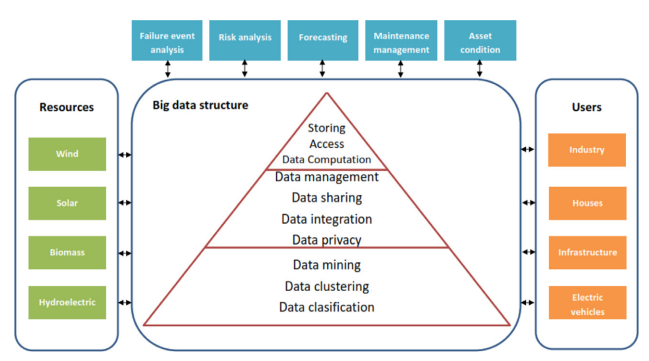
\includegraphics[width=1\textwidth]{img/teoria/bigdata2.png}
  \caption{Infraestructura de \textit{Big Data} enfocada al ámbito de las \gls{sg}s \cite{stab}}
  \label{fig:bigdata2}
\end{figure}

Para implementar esta infraestructura es preciso hacer uso de un entorno de computación en nube. Dentro de este contexto, las grandes tecnológicas como Google, Amazon y Microsoft han puesto sus esfuerzos en los últimos años en desarrollar y optimizar sus propios entornos de nube con el fin de integrar toda la gestión y análisis del \textit{Big Data} en una plataforma. A modo de aportar una mayor comprensión de su funcionamiento, se representa en la Figura \ref{fig:bigdata} un esquema de los servicios de nube disponibles.

\begin{figure}[h!]
  \centering
  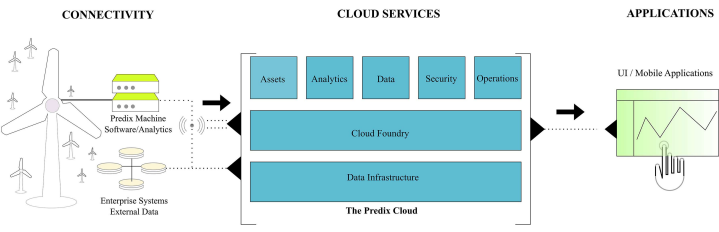
\includegraphics[width=1\textwidth]{img/teoria/bigdata.png}
  \caption{Plataforma de análisis de \textit{Big Data} en el entorno de \gls{sg}s \cite{bigdata}}
  \label{fig:bigdata}
\end{figure}

\vspace{3mm}

La computación en la nube se basa en el concepto de virtualización, el cual se puede definir como la tecnología que permite la creación de diferentes entornos virtuales aislados a partir de los recursos hardware disponibles y con independencia de este. Los proveedores de servicios emplean la virtualización para crear múltiples \gls{vm} y ofrecer recursos, como pueden ser el almacenamiento, la potencia de procesamiento o las aplicaciones de la nube, como diferentes servicios virtualizados. Esto aporta las siguientes ventajas a la computación en nube \cite{bigdata} \cite{virt}:

\begin{itemize}
  \item Escalabilidad: Se pueden aumentar o reducir recursos de la nube según las necesidades en cada instante temporal. Los usuarios consiguen un autoprovisionamiento de los recursos, ya que pueden desplegar instancias virtuales cuando lo deseen de forma manual o automática.
  \item Flexibilidad: Se ofrecen muchas posibilidades de configuración de los servicios de la nube.
  \item Interoperabilidad: Se emplean Interfaces de Programación de Aplicaciones (del ingles \gls{api}) para integrar plataformas y aplicaciones heterogéneas. El objetivo es soportar la comunicación entre las mismas y que se produzca una interpretación de los datos de forma correcta. Por ello, también se estandarizan los protocolos para que sean comunes. 
  \item Seguridad: Las plataformas de servicios de nube ofrecen un gran nivel de seguridad e implementan medidas como la encriptación de los datos y restricción de acceso o de permisos. Además, el aislamiento de los recursos y de las aplicaciones en diferentes \gls{vm} permite coonfigurar e implementar diferentes políticas de seguridad según las necesidades.
  \item Ahorro de costes: Se implementa un modelo de pago por uso en función de los recursos que se han consumido y se evita la inversión inicial necesaria para la instalación de una infraestructura física, además de su mantenimiento en el tiempo (CAPEX y OPEX).
  \item Disponibilidad: Se garantiza el acceso a los servicios y la confiabilidad de los mismos. Para ello, implementa técnicas de redundancia y aporta una buena toleracia a fallos.
\end{itemize}









\vspace{3mm}









%hablar de mineria de datos -> 3.2 datos inciertos (vacios y tal), 3.4 y 3.5



%stab

%Over the past few years, big data tools have been adopted by
% many major companies in the power industry such as IBM, Siemens,
% General Electric and Oracle (Arenas-Martinez et al., 2010). According to Li et al. (2012), about 85% of the processing tasks of big
% data can be delayed by a day. Hence, even if the energy output is
% time-varying and intermittent, it can be leveraged for processing the
% delayed datasets. Every day, more Terabytes of data emerge at the
% energy data center. Hence, it has become crucial to adopt big data
% technology to extract information from the multiple and diverse data
% sources through novel data centers (Liu et al., 2012). Through BDA, it
% would be possible to understand the behavior of energy consumption,
% which would help to improve energy efficiency and also promote the
% concepts of sustainability (Koseleva & Ropaite, 2017; Marmaras et al.,
% 2017; Mostafa & Negm, 2018).





%%bigdata

% 2.2 Industry perspective
% Even though the information technology related companies have
% achieved substantial success in the field of big data analytics,
% electrical industries are at the beginning stage to deploy big data. A
% few industries including Siemens, GE, ABB, OSI-Soft, and so on
% are developing big data platform and analytics for power grids. An
% account of a few commercially available platforms is provided here
% as a sample only and by no means is intended to be exhaustive.
% Siemens has developed a big data platform, called EnergyIP
% Analytics, which adds big data to smart grid application and
% provides insights on the management of big data for providing
% various grid services to electric utilities and grid operators [40].
% Siemens is currently integrating utility operations and data
% management technologies that could potentially be tapped for grid
% data analytics. This grid analytics platform can allow utilities to
% utilise big data for multiple functionalities, including home energy
% management, grid energy management, and predictive/corrective
% controls [40]. EnergyIP Analytics has already been used by more
% than 50 utilities with a total of 28 million installed smart devices
% [41].
% Similarly, GE has developed an industrial IoT platform, called
% PREDIX, to consolidate data from existing grid management
% systems, smart meters, and grid sensors [42]. In addition, Grid IQ
% Insight, a cloud-based big data analytics architecture, which utilises
% PREDIX platform, is developed to integrate big data analytics to
% grid applications [43]. Native data collected from Grid IQ Insight
% are stored in Data Lake that could be tapped for several grid
% applications [44]. In fact, these initiatives and developments
% support multiple grid applications ranging from real-time grid
% monitoring, distribution automation, home energy management,
% and ancillary services. As illustrated in Fig. 7, a concept of edgcomputing, whereby computational intelligence is connected at theedge of the data source, has been introduced by GE in its Grid IQInsight.
%ABB is integrating cloud computing and big data analytics
% intended for future power grid applications. ABB has developed an
% intelligent big data platform, called ABB Asset Health Center,
% which provides solutions for processing big data for smart grid
% applications [45]. In fact, ABB's Asset Health Center embeds
% equipment monitoring and systems expertise to establish end-toend asset management, business processes for reducing costs,
% minimising risks, improving reliability, and optimising operations
% across the electric utility [45]. In addition, OSI-Soft PI system,
% which is one of the most widely deployed database and analytics
% system, has been contributing to unveil the power of big data
% analytics to electric utilities. Smart asset management platform has
% introduced by OSI-Soft for the purpose of real-time monitoring of
% asset health [46].
% The aforementioned industries are offering utilities a way to
% gain a core understanding of what is the state of grid devices, and
% developing a launching pad for smart grid big data analytics
% applications over time. The next step for the industries is to
% effectively integrate prognosis and diagnosis into big data analytics
% framework so as to facilitate utilities to provide situational
% awareness, informed predictive decisions, condition monitoring,
% health management of critical grid infrastructure, and supporting
% grid functionalities.





















%ver (teoria)%20Smart-grid-based-big-data-analytics-using-machine-learning-and-artificial-intelligence-a-survey.pdf



